\documentclass[
11pt,%
tightenlines,%
twoside,%
onecolumn,%
nofloats,%
nobibnotes,%
nofootinbib,%
superscriptaddress,%
noshowpacs,%
centertags]%
{revtex4}
\usepackage{ljm}
\usepackage{listings}
\usepackage{amsmath}

\lstset{
language=C++,
basewidth=0.5em,
xleftmargin=45pt,
xrightmargin=45pt,
basicstyle=\small\ttfamily,
keywordstyle=\bfseries\underbar,
numbers=left,
numberstyle=\tiny,
stepnumber=1,
numbersep=10pt,
showspaces=false,
showstringspaces=false,
showtabs=false,
frame=trBL,
tabsize=2,
captionpos=t,
breaklines=true,
breakatwhitespace=false,
escapeinside={\%*}{*)}
}

\begin{document}

\titlerunning{TODO}
\authorrunning{Rybakov}

\title{TODO}

\author{\firstname{A.~A.}~\surname{Rybakov}}
\email[E-mail: ]{rybakov@jscc.ru, rybakov.aax@gmail.com}
\affiliation{Joint Supercomputer Center of the Russian Academy of Sciences -- branch of Scientific Research Institute of System Analysis of the Russian Academy of Sciences, Leninsky prospect 32a, Moscow, 119334, Russia}

\firstcollaboration{(Submitted by TODO)} % Add if you know submitter.
%\lastcollaboration{ }

\received{TODO}

\begin{abstract}
TODO
\end{abstract}

\subclass{TODO} % Enter 2010 Mathematics Subject Classification.

\keywords{TODO}

\maketitle

\section{Introduction}

TODO

\section{TODO}

\begin{figure}
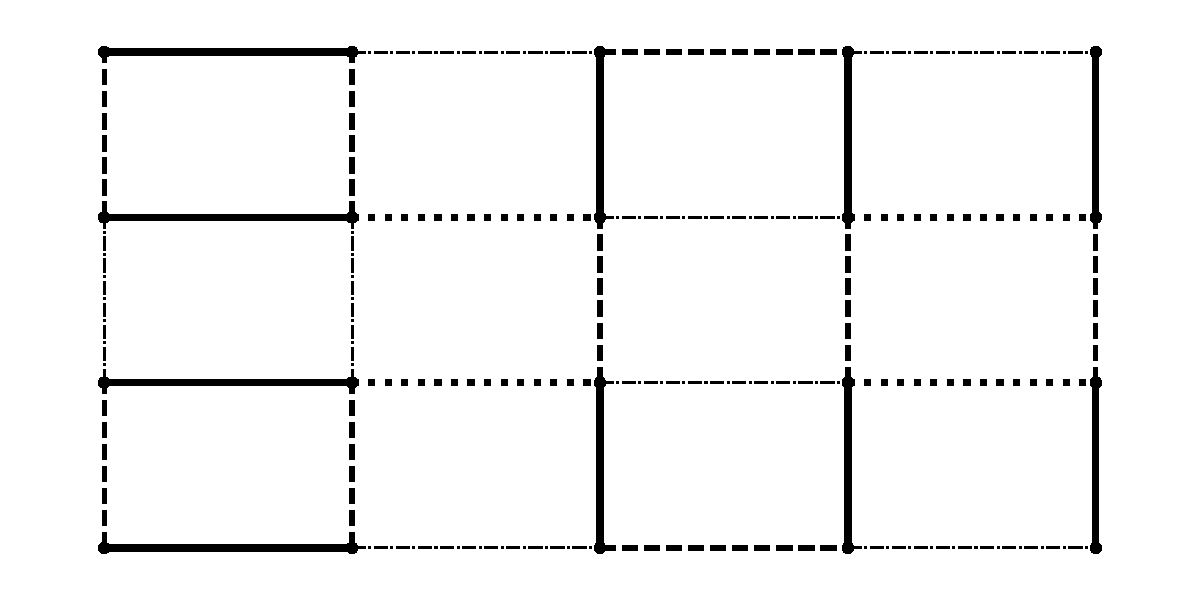
\includegraphics[width=0.8\linewidth]{pics/s2d.pdf}
\end{figure}

\begin{figure}
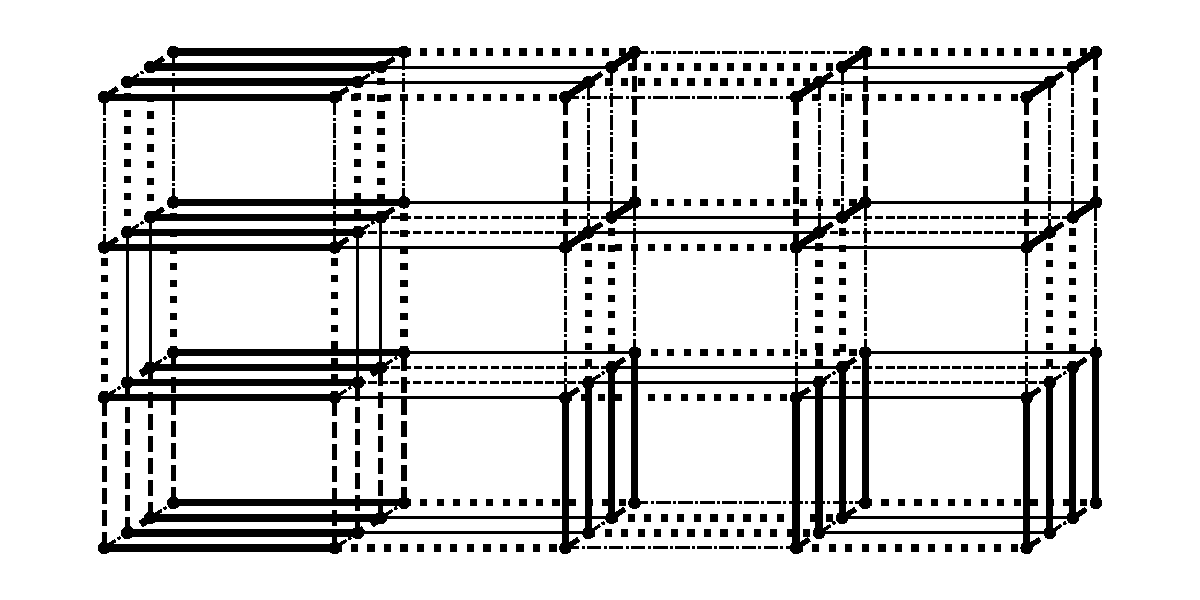
\includegraphics[width=0.8\linewidth]{pics/s3d.pdf}
\end{figure}

\section{TODO}

\begin{figure}
	\subfigure[]{\label{fig:u2d_col01}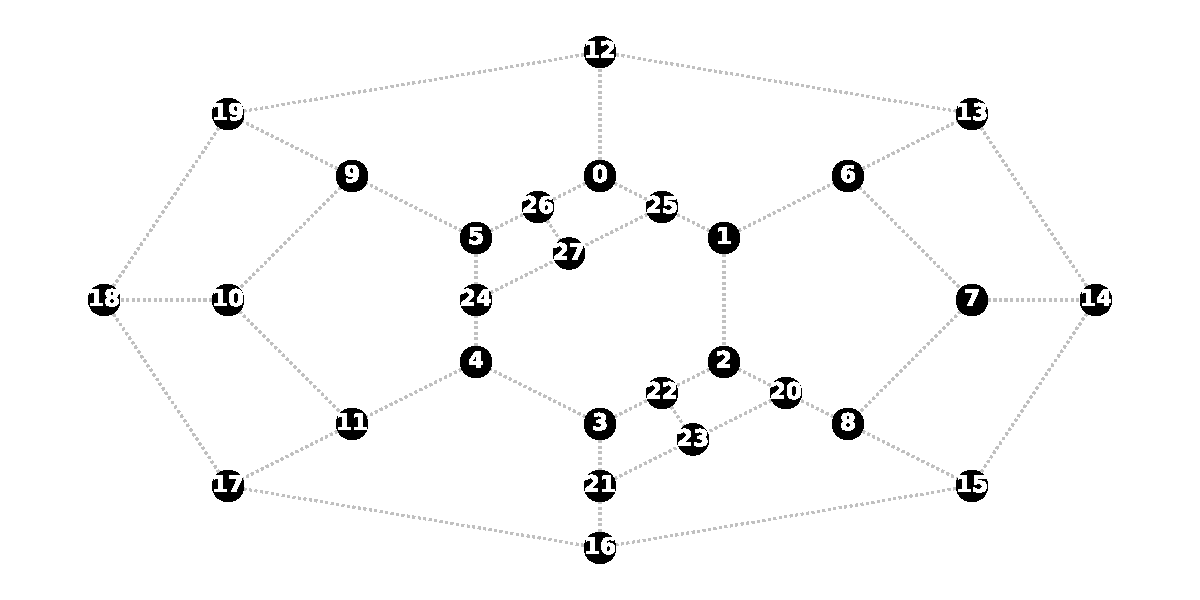
\includegraphics[width=0.48\linewidth]{pics/u2d_col01.pdf}}
	\subfigure[]{\label{fig:u2d_col02}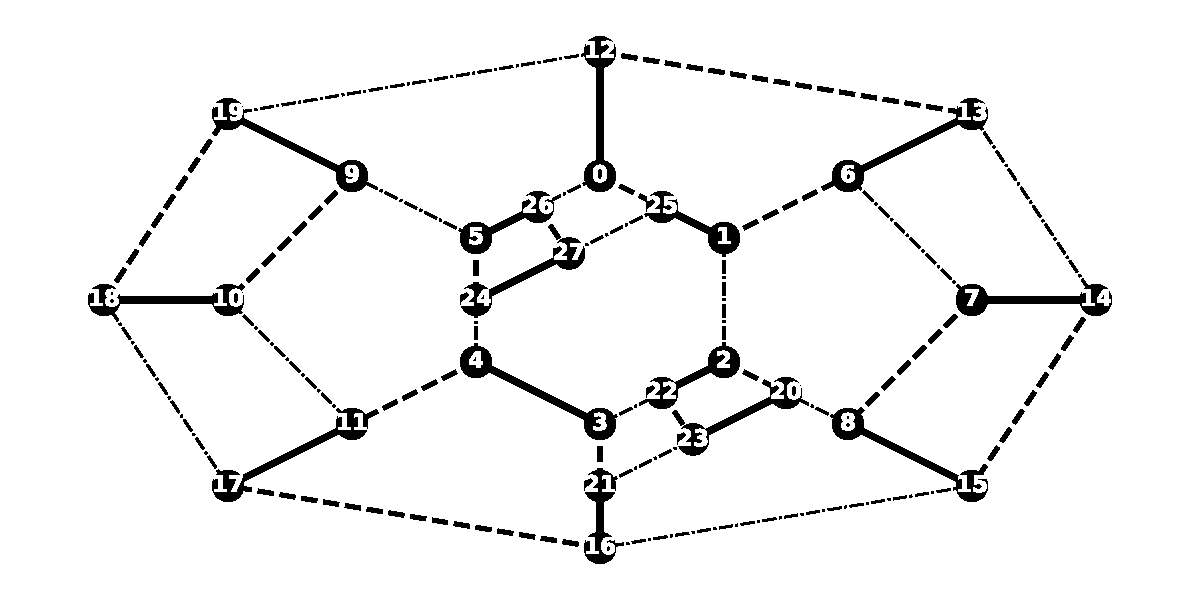
\includegraphics[width=0.48\linewidth]{pics/u2d_col02.pdf}}
	\subfigure[]{\label{fig:u2d_col03}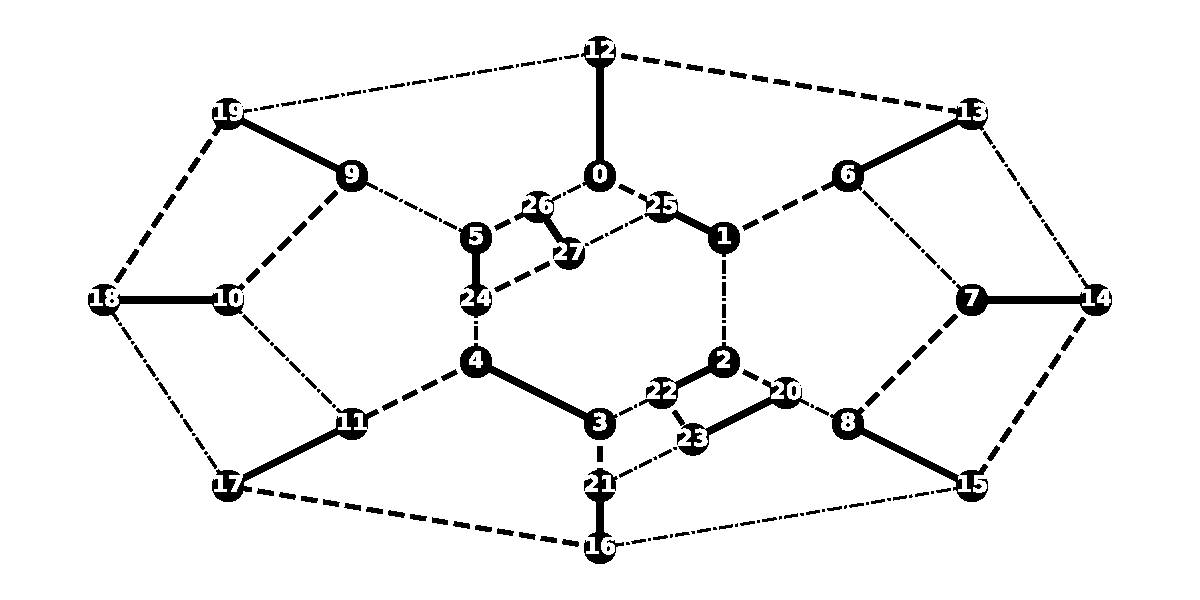
\includegraphics[width=0.48\linewidth]{pics/u2d_col03.pdf}}
	\subfigure[]{\label{fig:u2d_col04}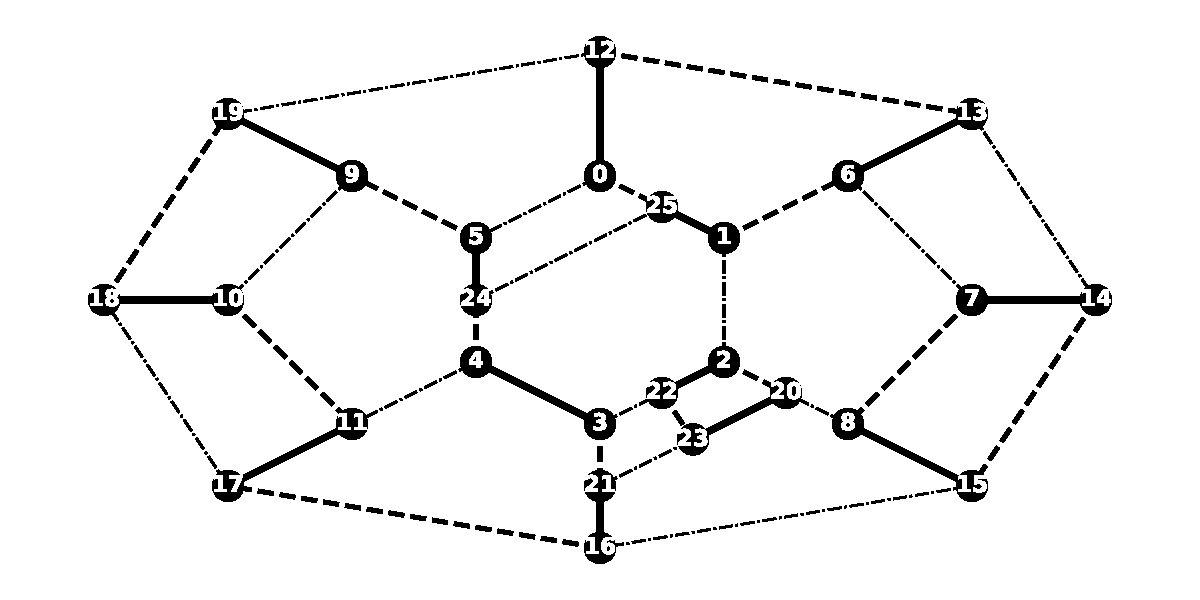
\includegraphics[width=0.48\linewidth]{pics/u2d_col04.pdf}}
	\subfigure[]{\label{fig:u2d_col05}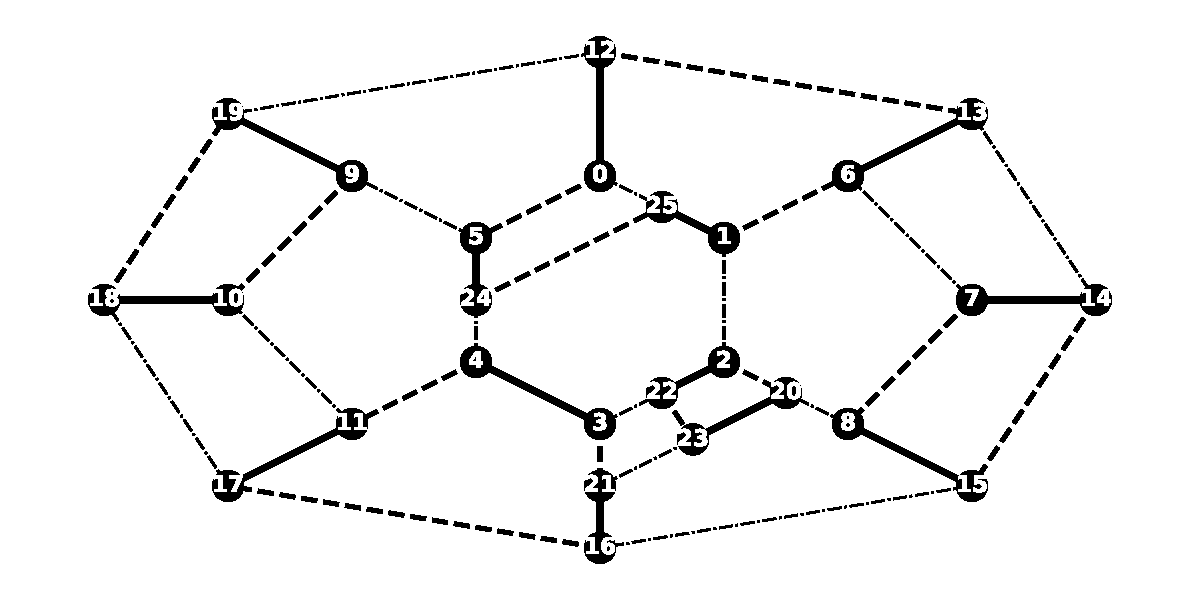
\includegraphics[width=0.48\linewidth]{pics/u2d_col05.pdf}}
	\subfigure[]{\label{fig:u2d_col06}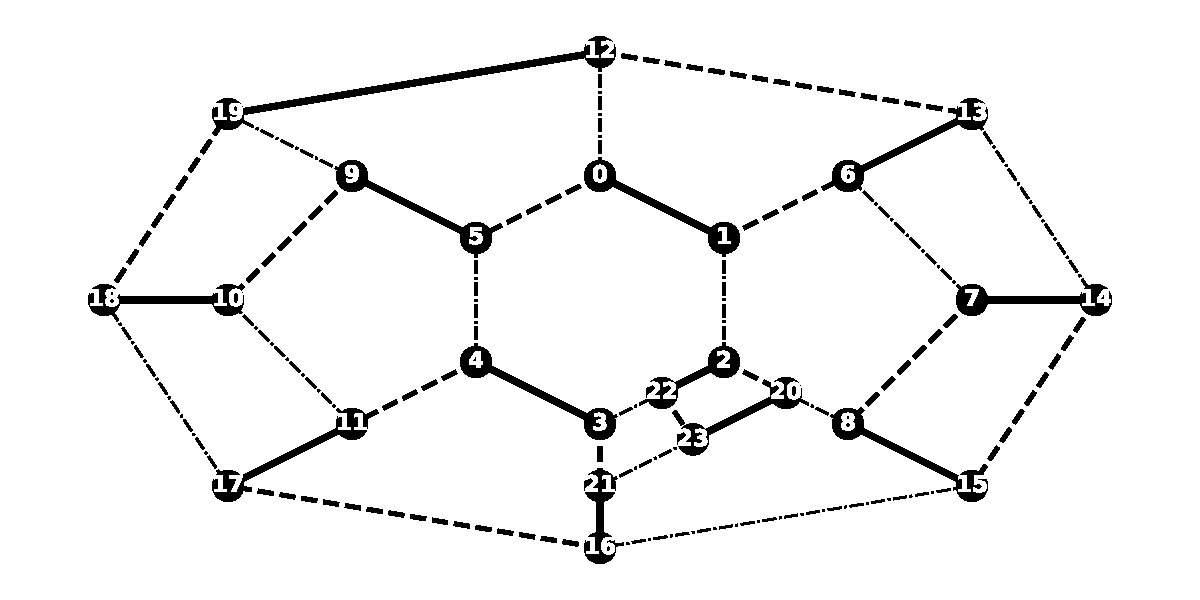
\includegraphics[width=0.48\linewidth]{pics/u2d_col06.pdf}}
	\subfigure[]{\label{fig:u2d_col07}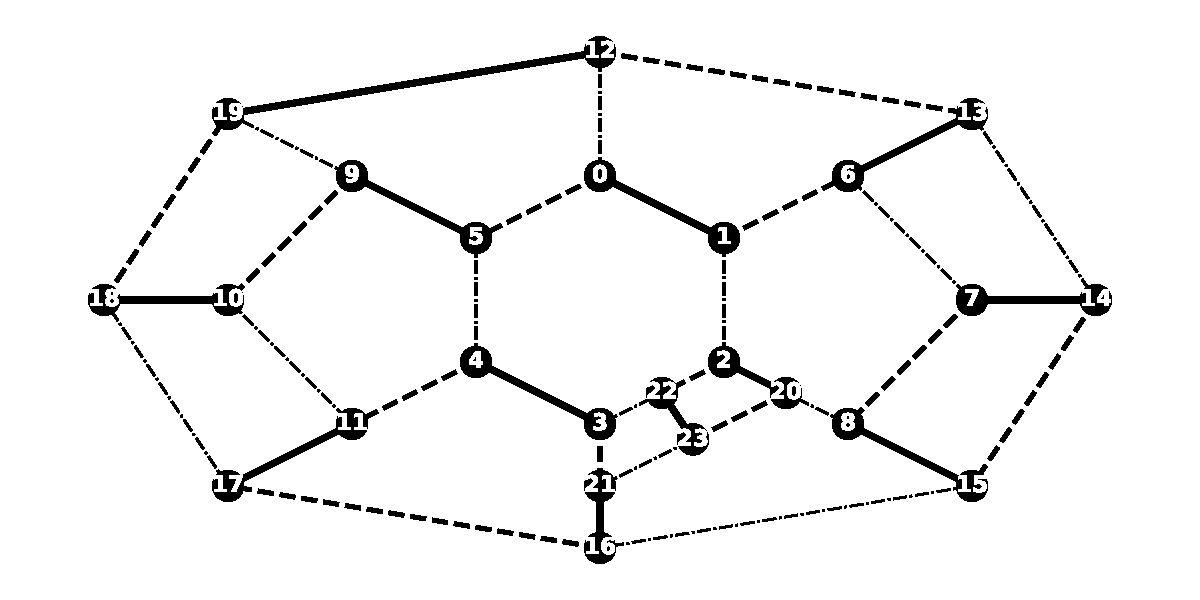
\includegraphics[width=0.48\linewidth]{pics/u2d_col07.pdf}}
	\subfigure[]{\label{fig:u2d_col08}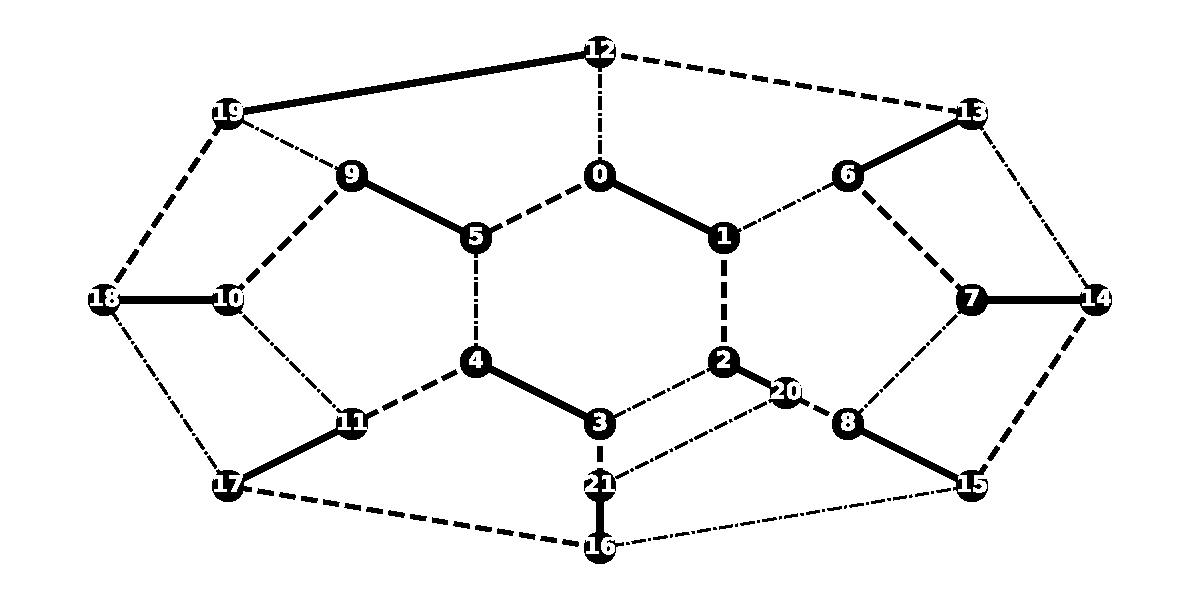
\includegraphics[width=0.48\linewidth]{pics/u2d_col08.pdf}}
	\subfigure[]{\label{fig:u2d_col09}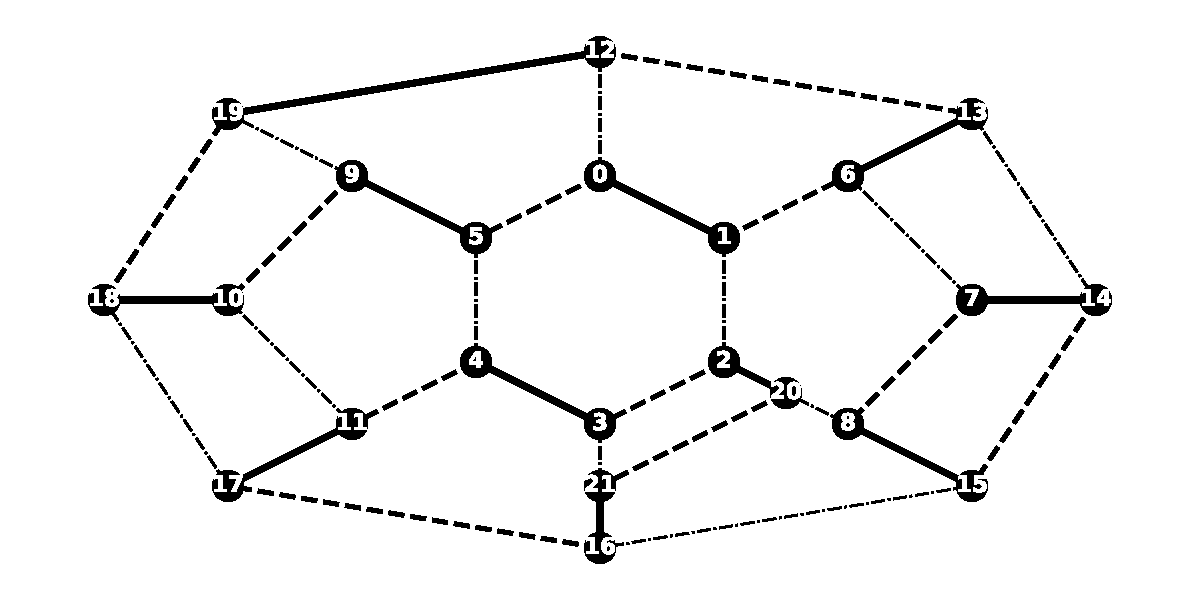
\includegraphics[width=0.48\linewidth]{pics/u2d_col09.pdf}}
	\subfigure[]{\label{fig:u2d_col10}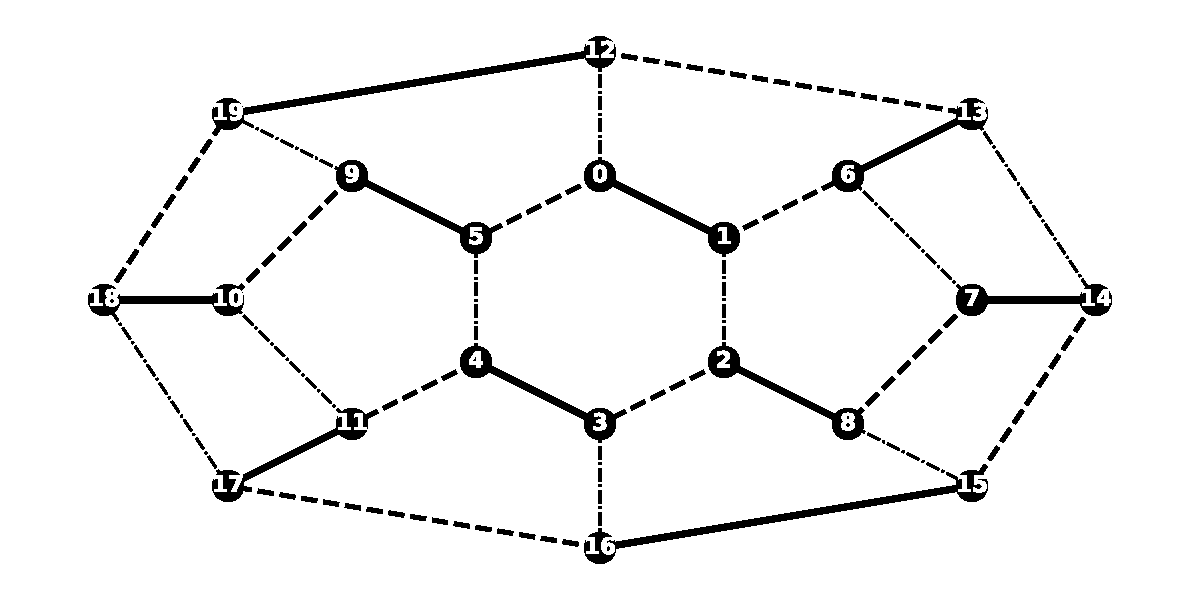
\includegraphics[width=0.48\linewidth]{pics/u2d_col10.pdf}}
\caption{TODO}
\end{figure}

\section{TODO}

\begin{figure}
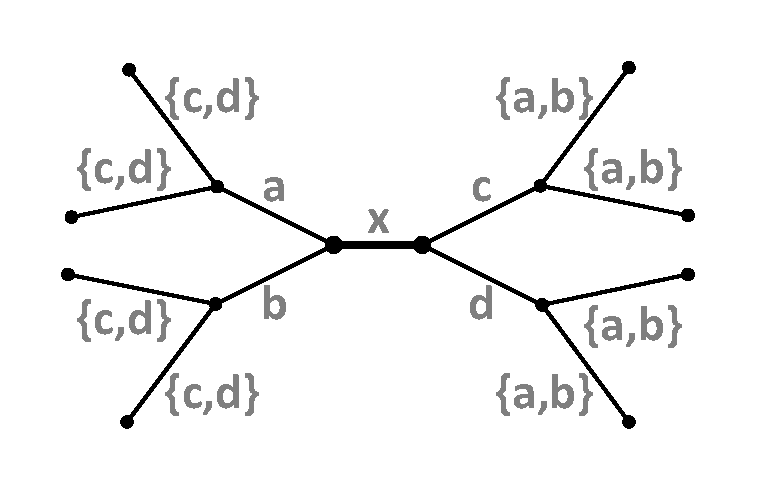
\includegraphics[width=0.8\linewidth]{pics/recoloring_neighborhood.pdf}
\end{figure}

\begin{figure}
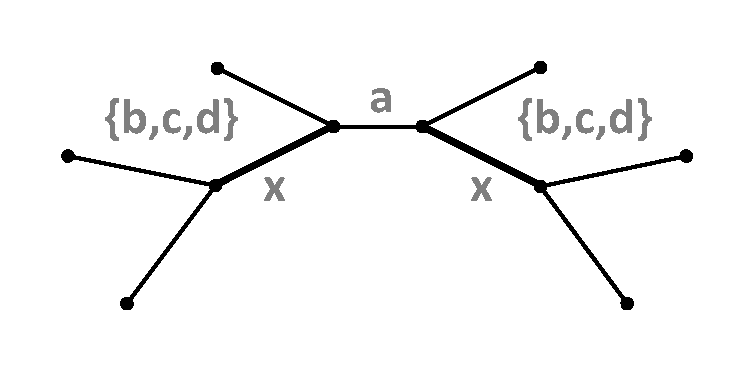
\includegraphics[width=0.8\linewidth]{pics/recoloring_doublex.pdf}
\end{figure}

\begin{figure}
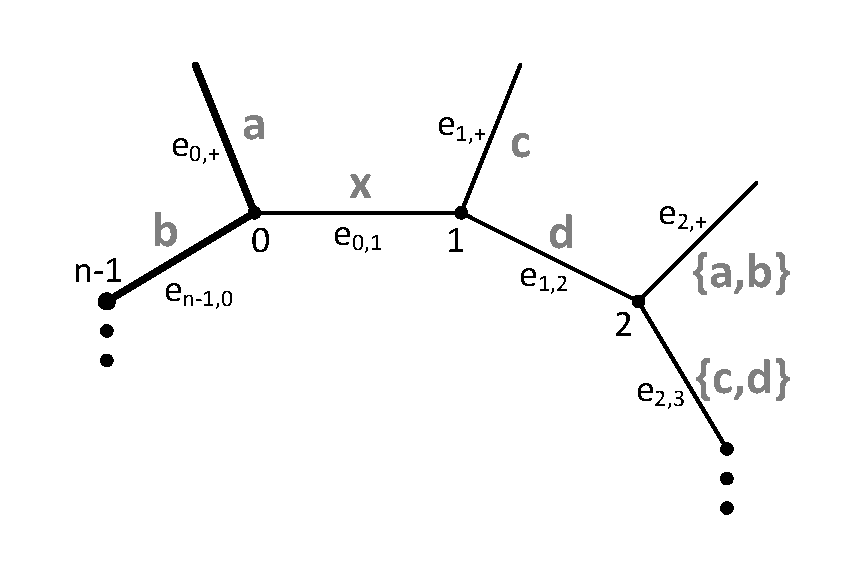
\includegraphics[width=0.8\linewidth]{pics/recoloring_cycle.pdf}
\end{figure}

\section{Conclusion}

TODO

\begin{acknowledgments}
TODO
\end{acknowledgments}

\begin{thebibliography}{99}

% 1. Intruduction.

\bibitem{TODO}
\refitem{TODO}
TODO.

\end{thebibliography}

\end{document}
